\chapter{Application}
\label{chap:application}
%#############################################################################################

In this chapter, we are trying to apply the algorithms that are described and implemented in Chapter~\ref{implementation} to various datasets: \textit{usps}, \textit{banana}, \textit{fishbowl}, \textit{swissroll} and \textit{flatroll}.


%#############################################################################################
\section{Assignment 3: ROC Curve}
\label{assignment3}

This assignment asks us to apply \textit{PCA} to the \textit{usps} data set and visualizing the results. The \textit{usps} data set consists of 2007 images with the dimension of \textit{16 x 16}. The images are hand-written digits of zero to nine, which can be viewed as classes. Firstly, i separate the data set according to each digit into ten classes and then applied \textit{PCA} to each class. The \textit{PCA} was applied to the original data set and noisy data set.



\begin{figure}[h!]
	\centering
	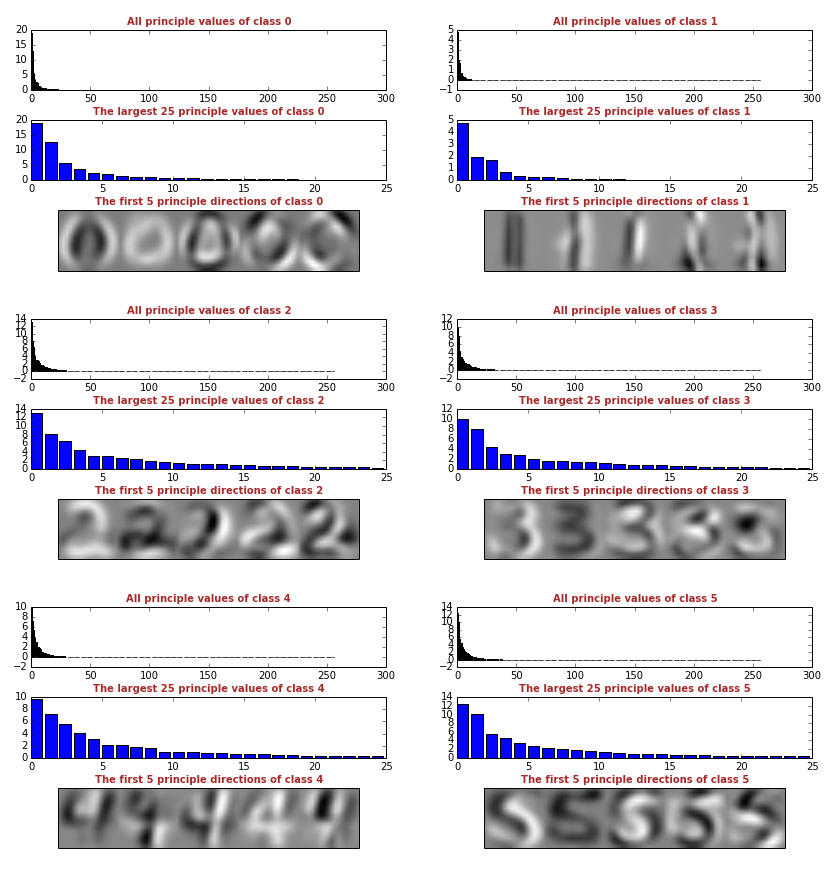
\includegraphics[scale=0.4983]{normalpca_0-5}
	\caption{Principal components of usps original data set for class 0 - 5}
	\label{fig:pcaOriginal05}
\end{figure}


%#############################################################################################
\section{Assignment 4: Kernel Ridge Regression}
\label{assignment4}

In this assignment, the $\gamma$-index method is utilized to detect outliers and applied it to the \textit{banana} data set. The positive class of the data set is used as \textit{inliers}, to which the negative class is added as outliers. The $\gamma$-index is then used to detect outliers with contamination rates of 1\%, 5\%, 10\% and 25\% relative to the positive class. Figure~\ref{fig:bananacomplete} shows the complete original data set, both positive and negative class, whereas Figure~\ref{fig:bananacontaminated} shows the contaminated data set.

\begin{figure}[h!]
	\centering
	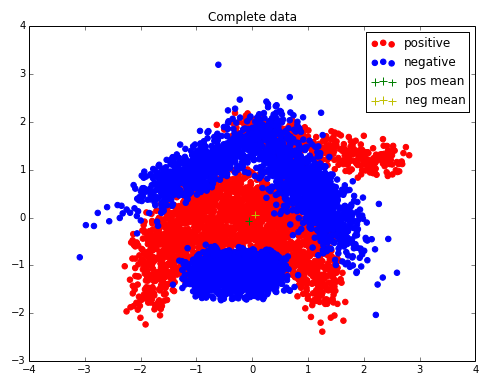
\includegraphics[scale=0.4983]{banana_complete}
	\caption{Both positive and negative of banana data set, including the mean of both classes}
	\label{fig:bananacomplete}
\end{figure}

\begin{figure}[h!]
	\centering
	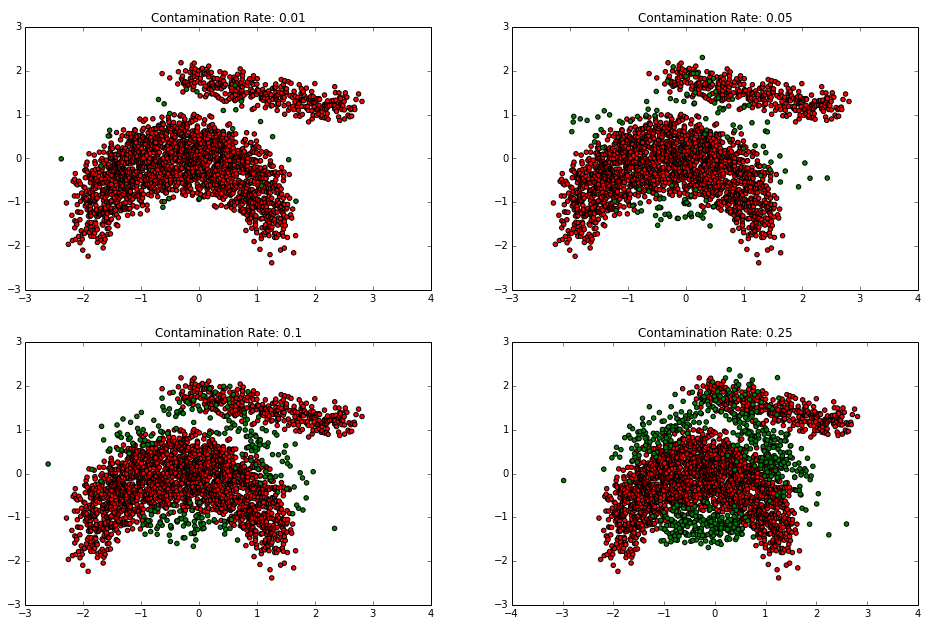
\includegraphics[scale=0.4983]{banana_contaminated}
	\caption{Contaminated banana data set with contamination rate of 1\%, 5\%, 10\% and 25\%}
	\label{fig:bananacontaminated}
\end{figure}

There are three methods that should be used to detect the outliers: (a) the $\gamma$-index with $k=3$, (b) the $\gamma$-index with $k=10$ and (c) the distance to the mean for each data point. All of the methods are then applied to the four contamination rates mentioned above. After that, the \textit{AUC} (area under the \textit{ROC}) should be calculated. Figure~\ref{fig:gammaboxplots} shows the boxplots that visualize the distribution of the \textit{AUC} values.

\begin{figure}[h!]
	\centering
	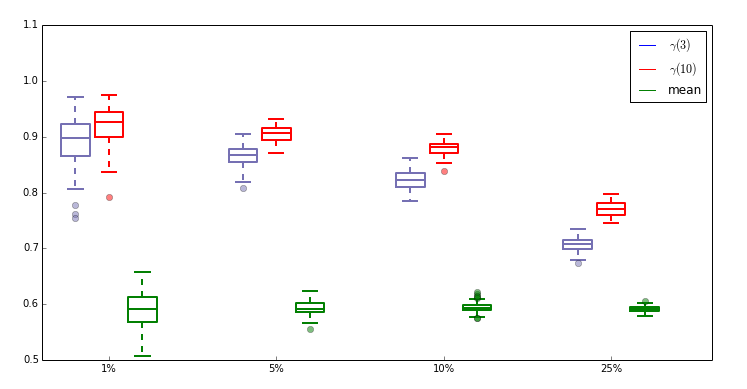
\includegraphics[scale=0.5583]{gamma_boxplots}
	\caption{Boxplots visualizing the distribution of the \textit{AUC} values}
	\label{fig:gammaboxplots}
\end{figure}

The boxplots show that the method using the distance to the mean for each data point performed quite bad, while both of the $\gamma$-index methods performed very well, especially for the data set with lower contamination rates. The $\gamma$-index with $k=10$ performed slightly better than the $\gamma$-index with $k=3$.
